\usetikzlibrary{arrows.meta,matrix,positioning}

\begin{frame}{predicting ret: extra copy of stack}
\begin{itemize}
    \item predicting ret --- ministack in processor registers
    \item push on ministack on call; pop on ret
    \item ministack overflows? discard oldest, mispredict it later
\end{itemize}
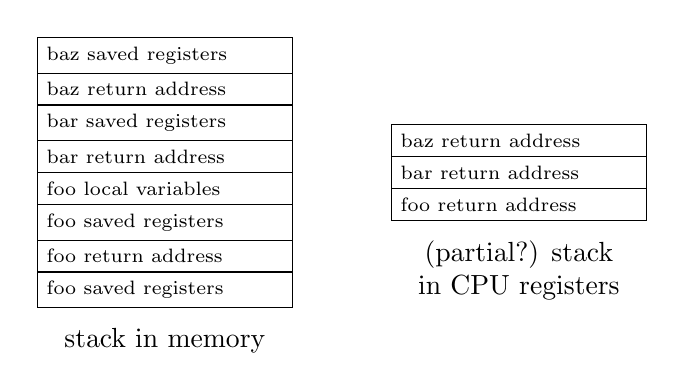
\begin{tikzpicture}
\matrix [matrix of nodes, nodes={draw,rectangle,row sep=-\pgflinewidth,font=\scriptsize, text width=3cm},
         label={-90:stack in memory}] (realStack) {
    baz saved registers \\
    baz return address \\
    bar saved registers \\
    bar return address \\
    foo local variables \\
    foo saved registers \\
    foo return address \\
    foo saved registers \\
 };

\matrix [matrix of nodes,row sep=-\pgflinewidth,nodes={draw,rectangle,font=\scriptsize,text width=3cm},
         label={[align=center]-90:(partial?) stack\\in CPU registers},right=1cm of realStack] (fakeStack) {
    baz return address \\
    bar return address \\
    foo return address \\
 };
\end{tikzpicture}
\end{frame}

\begin{frame}{4-entry return address stack}
\begin{tikzpicture}
    \tikzset{>=Latex}
    \matrix[tight matrix,
        nodes={minimum height=.5cm},
        row 1/.style={nodes={minimum height=1.65cm}},
        column 2/.style={nodes={text width=3cm,draw}},
        column 1/.style={nodes={text width=1cm,draw}},
        label={north:4-entry return address stack in CPU},
    ] (ras) {
        idx \& {saved \\ return \\ addresses} \\
        0 \& 0x12345 \\
        1 \& 0x44432 \\
        2 \& 0x44F92 \\
        3 \& 0x22331 \\
    };
    \node[anchor=east,draw,label={[align=center]north:current\\index}] (ras idx) at ([xshift=-1cm]ras.west) {1};
\draw[very thick,->,dotted] (ras idx) -- ++(.5cm, 0cm) |- (ras-3-1.west);
    \draw[very thick,->] (ras-3-2.east) -- ++(2cm, 0cm) node[right ] {next prediction for ret};
    \draw[very thick,<-] (ras-4-2.east) -- ++(1cm, 0cm) -- ++(0cm, -1cm) node[below,align=center] {next saved \\ return address \\ from call};
\end{tikzpicture}
\begin{itemize}
\item on \texttt{call}: increment index, save return address in that slot
\item on \texttt{ret}: read prediction from index, decrement index
\end{itemize}
\end{frame}
